\documentclass{article}%
\usepackage[T1]{fontenc}%
\usepackage[utf8]{inputenc}%
\usepackage{lmodern}%
\usepackage{textcomp}%
\usepackage{lastpage}%
\usepackage{graphicx}%
%
\title{Default}%
\author{Notepal}%
\date{\today}%
%
\begin{document}%
\normalsize%
\maketitle%
\section{Note1}%
\label{sec:Note1}%
\subsection{Page 1}%
\label{subsec:Page 1}%


\begin{figure}[h!]%
\centering%
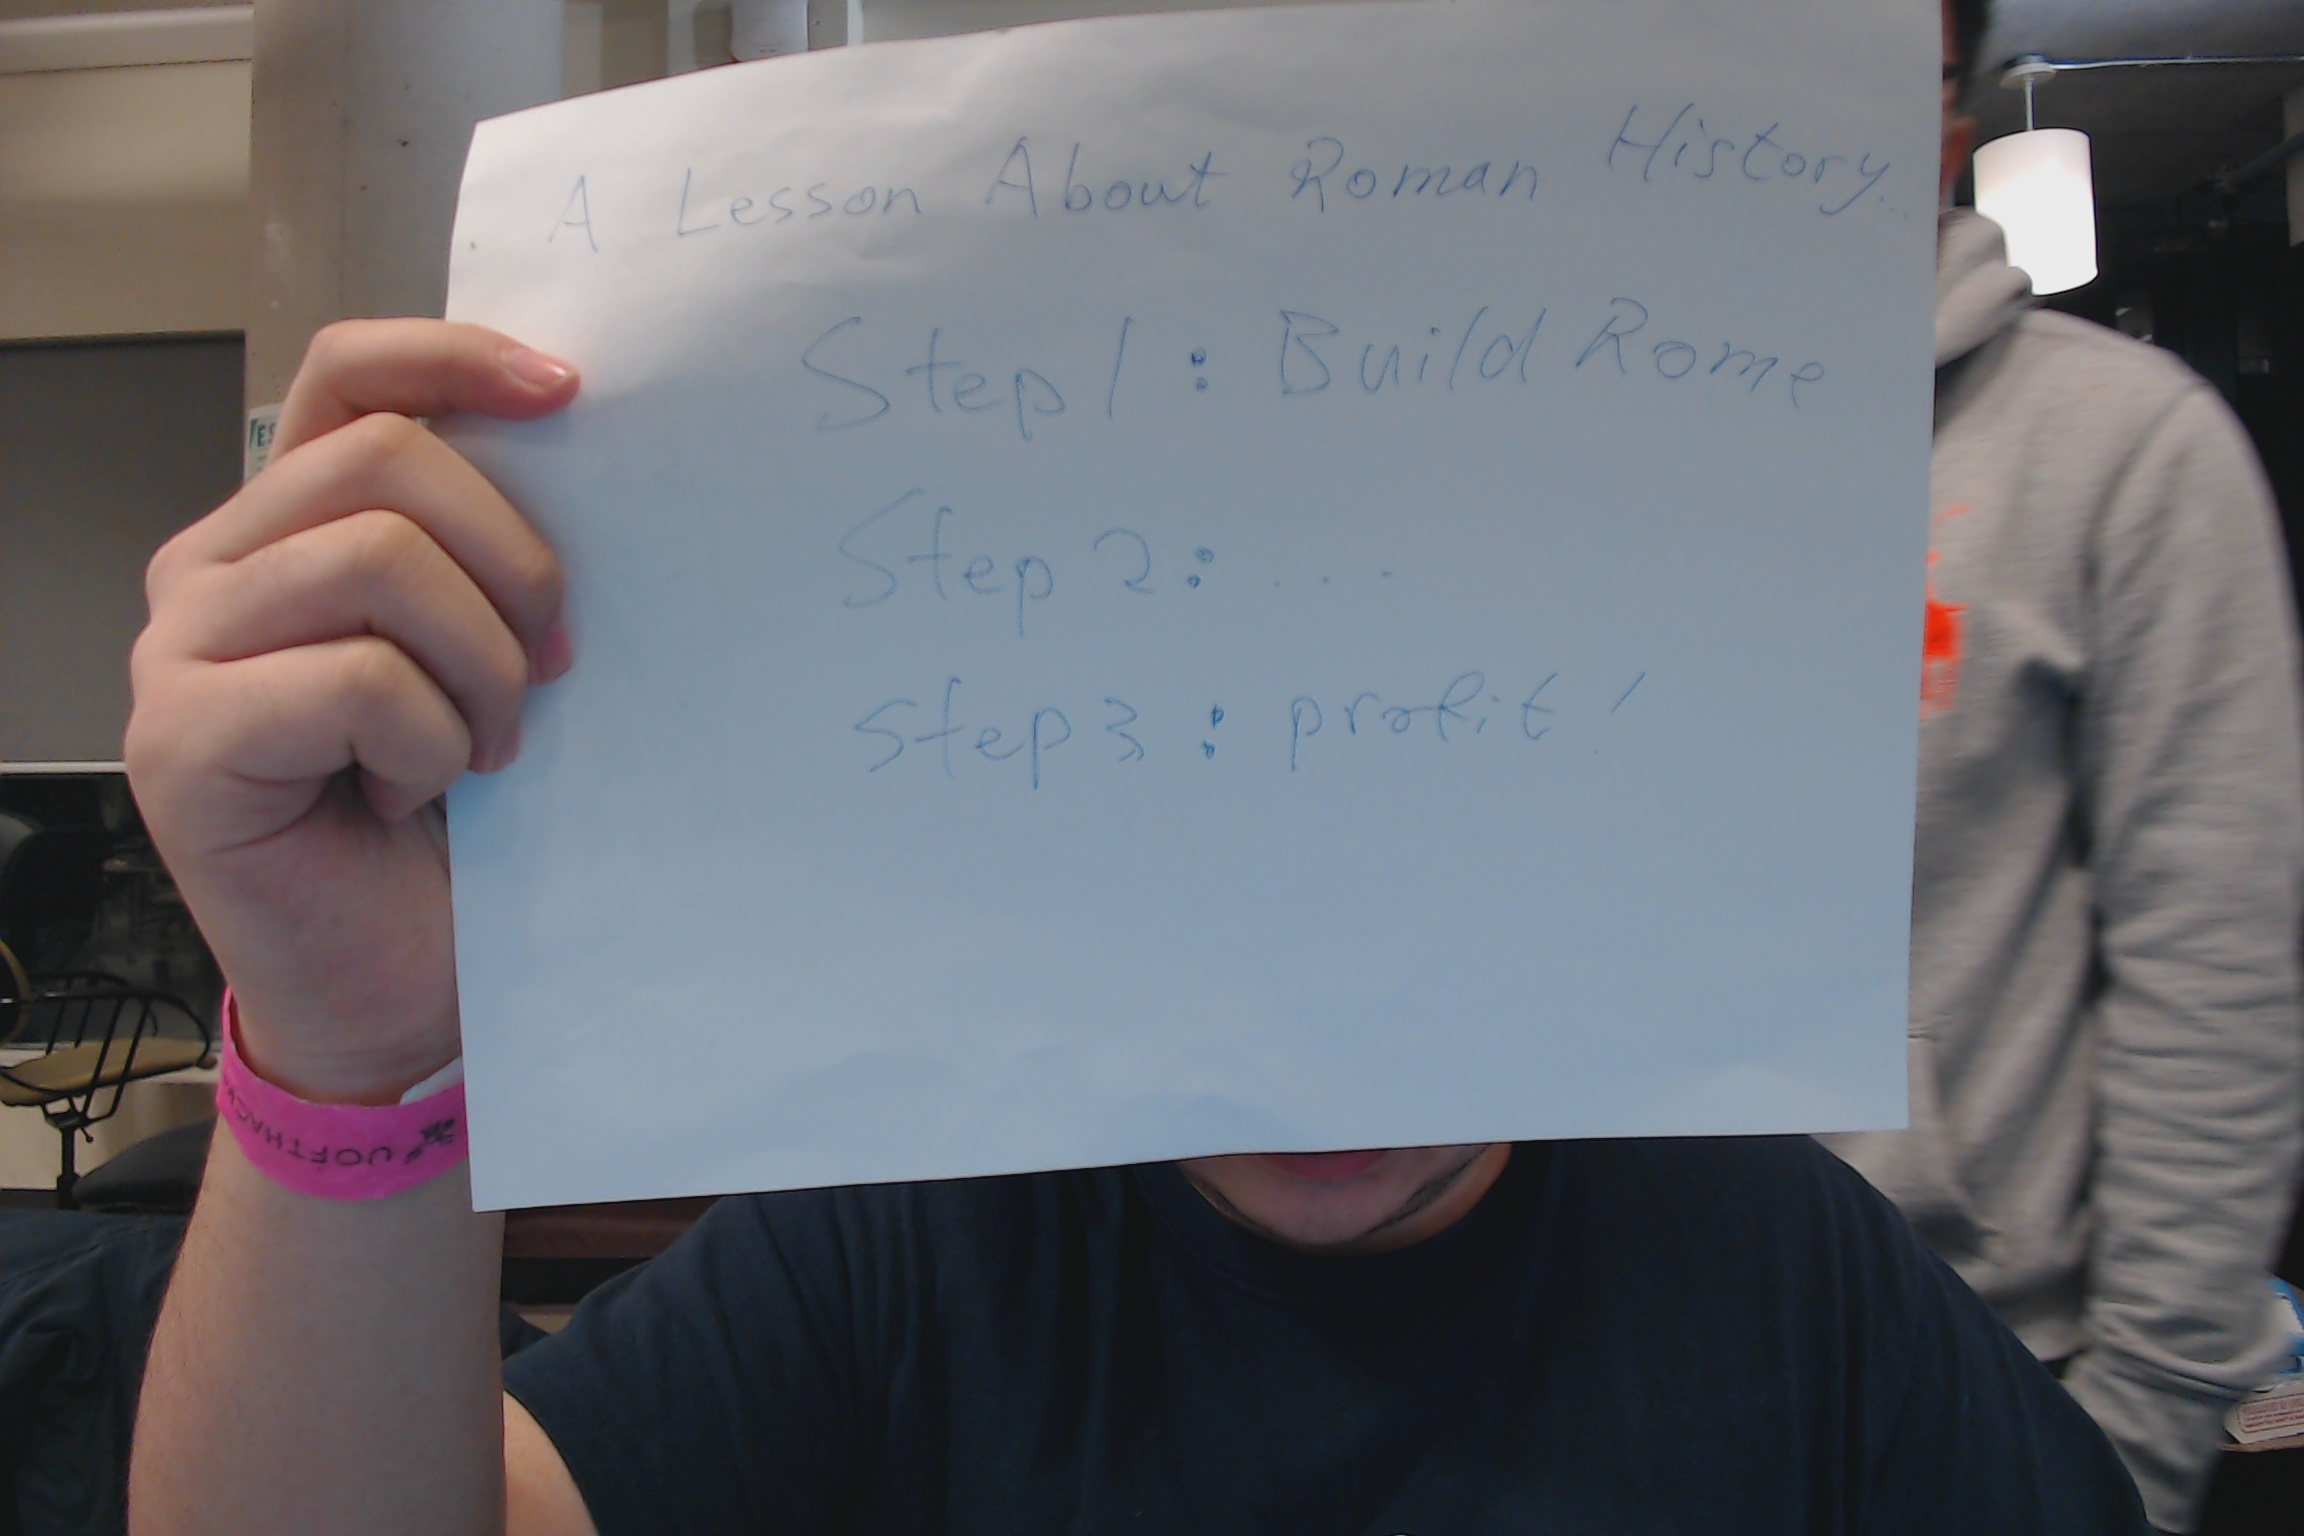
\includegraphics[width=300px]{../Notes/IntroductiontoDatabases/Note1/image1.jpg}%
\caption{Image 1}%
\end{figure}

%
Okay, good morning. Everyone today. We're going to talk a little bit about SQL and how we use it in a relational databases next page. \newline%

%
\subsection{Page 2}%
\label{subsec:Page 2}%


\begin{figure}[h!]%
\centering%
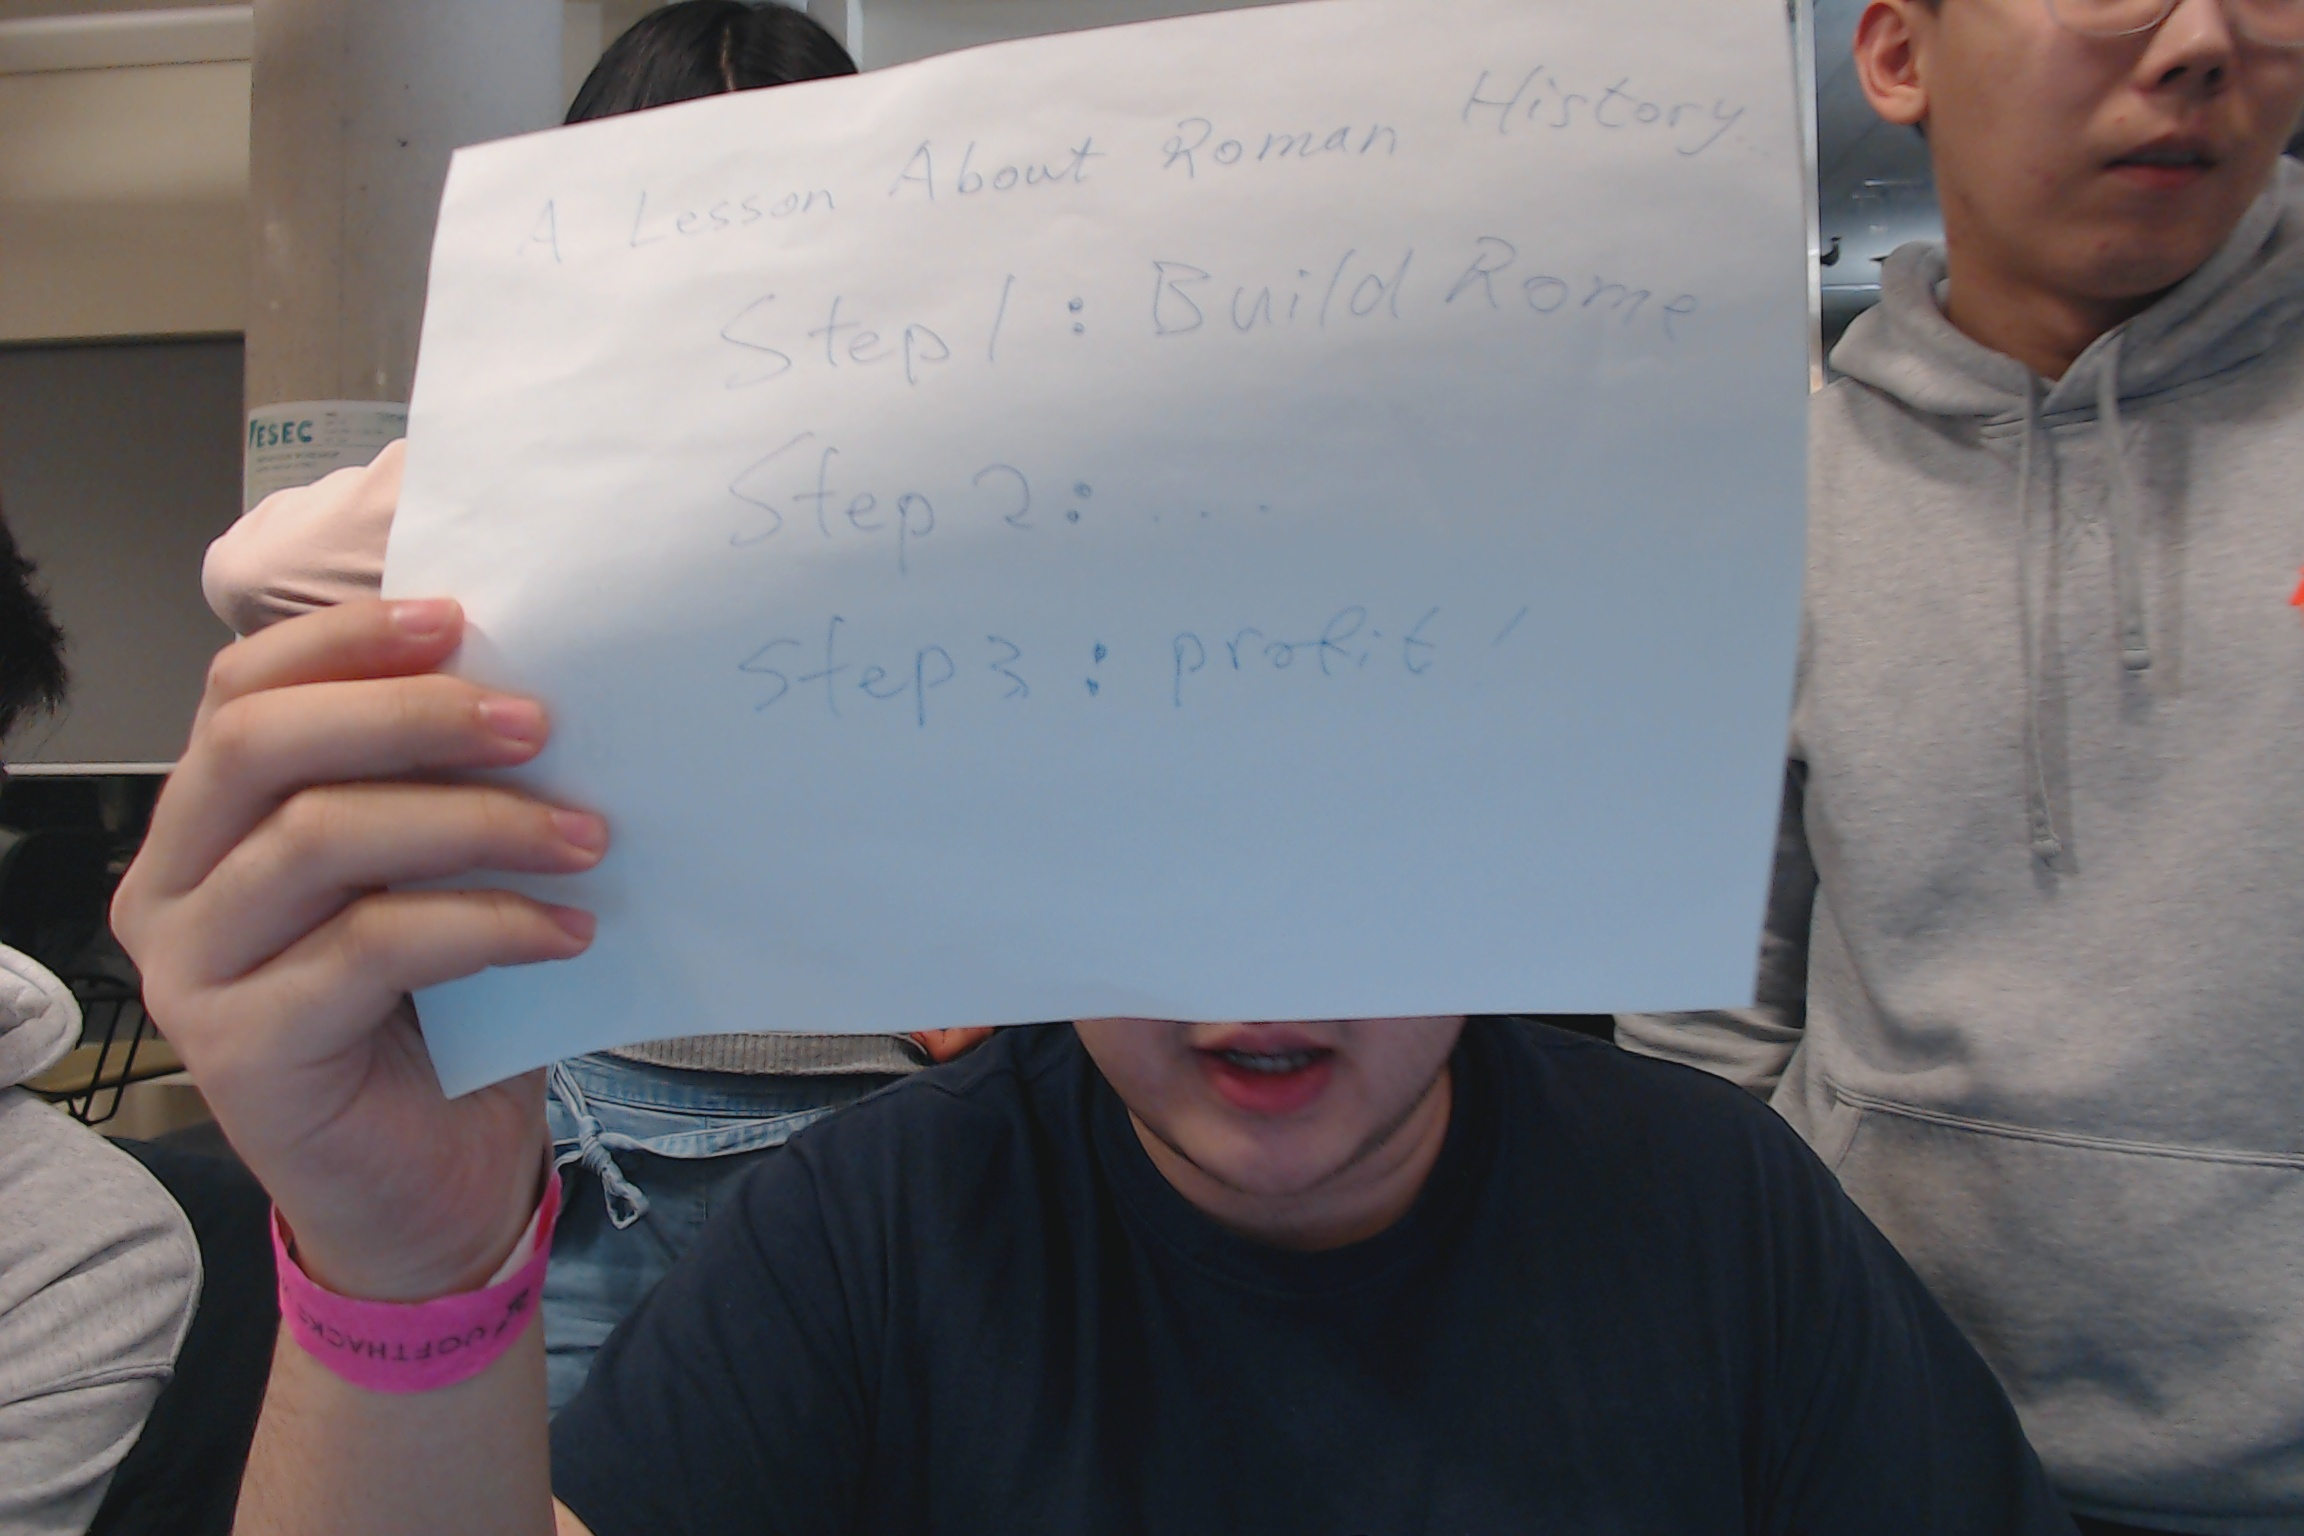
\includegraphics[width=300px]{../Notes/IntroductiontoDatabases/Note1/image2.jpg}%
\caption{Image 2}%
\end{figure}

%
Okay, let's continue talking about SQL. But specifically we want to start with relational{-}algebra see how that leads into SQL and \newline%
 Just keep forgetting what to say. That's why I make sure all. \newline%

%
\end{document}